\section{Data Analysis}
During the solution of this assignment I will not consider any additional data
sources, or external datasets. Consequently, I will use only the provided
MovieLens-100k dataset.

While the dataset contains a lot of additional metadata, I will use only the
most important fracture of it to build the analysis and solution for the given
task.

First and foremost, we can consider the genres of the movies in the dataset as
depicted on figure~\ref{fig:dataanalysis:genre_distr}.

\begin{minipage}{\linewidth}
    \centering% 
    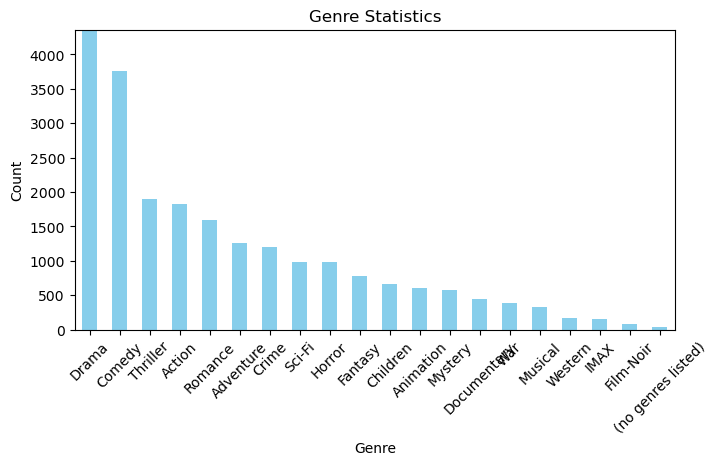
\includegraphics[scale=0.3]{assets/genre_distribution.png}% 
    \figcaption{Genres distribution}% 
    \label{fig:dataanalysis:genre_distr}% 
\end{minipage}

We can conclude, that the dataset is pretty imbalanced, which is itself a
problem. It is safe to assume that this distribution of the movies will affect
the final predictions of the solution. For instance, most probably the model
will try to propose dramas and it will be difficult to derive useful Noir
recommendations. For the sake of simplicity, I will ignore the imbalance.

\begin{minipage}{\linewidth}
    \centering% 
    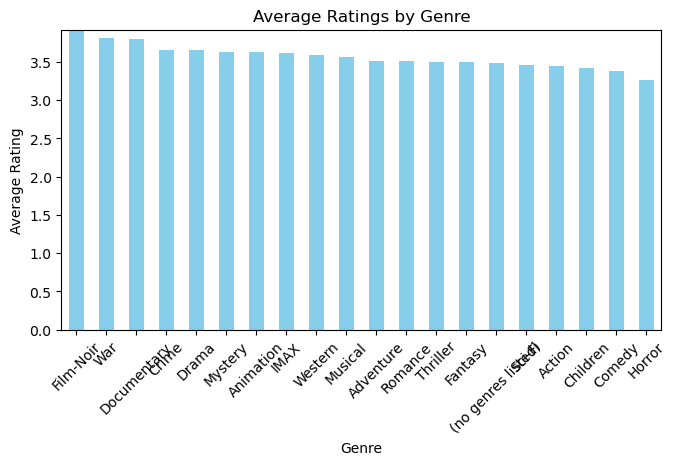
\includegraphics[scale=0.3]{assets/genre_rating.png}% 
    \figcaption{Average raiting by genre}% 
    \label{fig:dataanalysis:avg_genre_ratings}% 
\end{minipage}

Moreover, from figure~\ref{fig:dataanalysis:avg_genre_ratings} we can derive,
that popularity of the genre does not necessarily mean it's quality. For
instance, if we will consider comedy, which is the second popular genre, it's
overall rating is the second from the bottom. It represents the difficulty the
recommender system has to overcome. Learning the preferences is not enough as
general genre recommendation will lead to poor results.

\begin{minipage}{\linewidth}
    \centering% 
    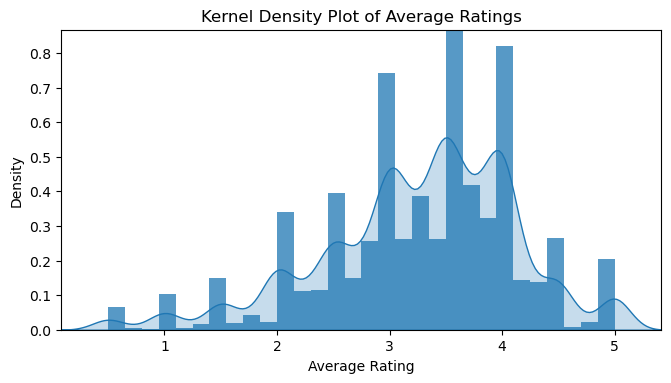
\includegraphics[scale=0.3]{assets/average_ratings_pretty.png}% 
    \figcaption{Average movie ratings}% 
    \label{fig:dataanalysis:avg_movie_ratings}% 
\end{minipage}

\end{multicols*}
\begin{minipage}{\linewidth}
    \centering% 
    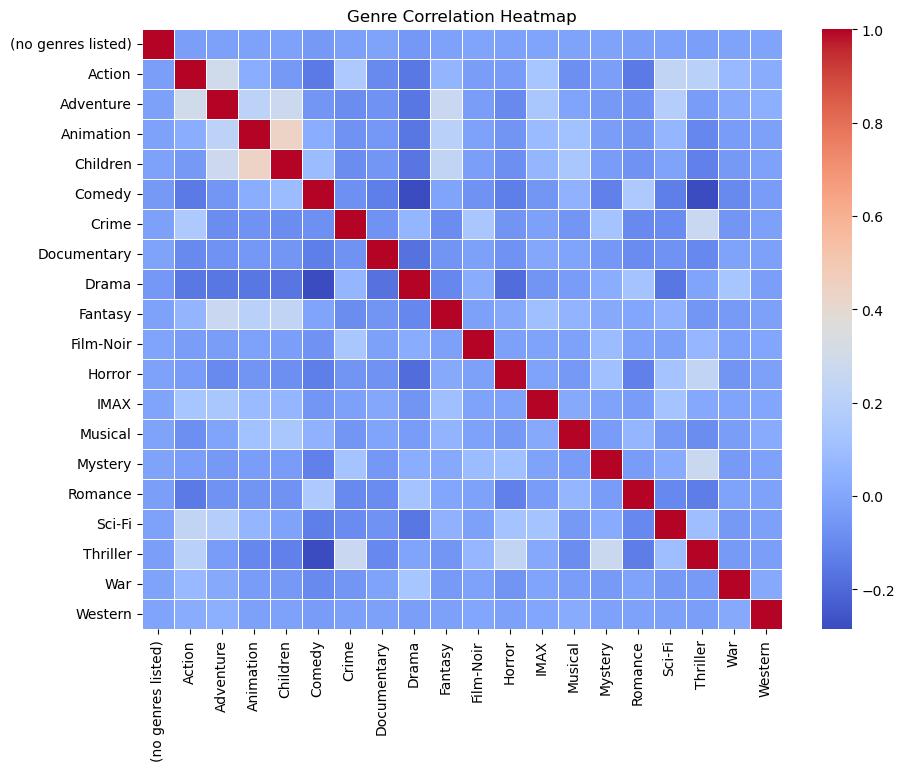
\includegraphics[scale=0.6]{assets/genre_corr_heatmap.png}% 
    \figcaption{Average genre ratings}% 
    \label{fig:dataanalysis:correlation}% 
\end{minipage}
\begin{multicols*}{2}

From user rating on figure~\ref{fig:dataanalysis:avg_movie_ratings} we can
learn interesting properties as well. For instance, the rating distribution
seem to be normal except some outliers. But these outlieres are not random as
well. They tend to reflect that users prefer to give \textit{pretty} numbers as
ratings. For instance, integer numbers, or half-numbers like \(1.5\) or
\(2.5\).

Moreover, candlesticks plots show that while Film-Noir tends to be very rare
genre, even lowest ratings are high. However, the horror movies tend to have
very large ratings gap. Even though most of the grades are relatively low,
leading to low average.

\begin{minipage}{\linewidth}
    \centering% 
    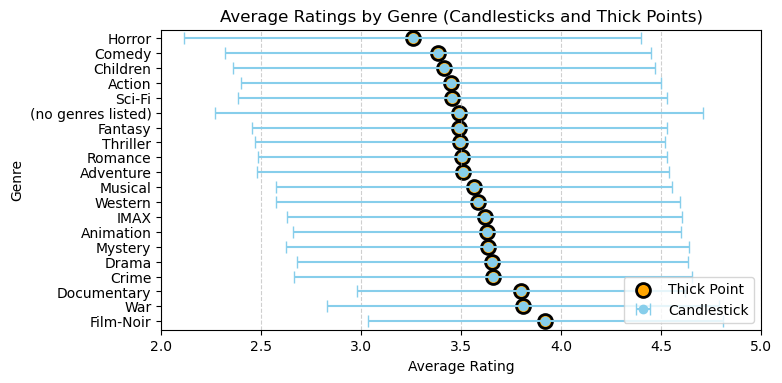
\includegraphics[scale=0.3]{assets/genre_candle_rating.png}% 
    \figcaption{Genres rating candles}% 
    \label{fig:dataanalysis:rating_candles}% 
\end{minipage}

Finally, we can consider the correlation data of the genres. This data mostly
reflects how the genres work along with each other. For instance, if a movie is
a comedy, it is most probably not a thriller, as well as children movies most
often tend to be animation.

The correlation data may seem redundant. However, carefully incorporating these
properties into the model, we can try to learn the correlation. For instance,
if a user prefers mostly comedy, probably model should not recommend thrillers
a lot.

Finally, successfully learning the properties we discovered in the data, we can
properly build the model, learning these patterns and improving overall
performance. Consequently, we can proceed to the model implementation in the
next chapter.

